\question[3]
Der Graph wird von Startknoten a aus mit Tiefensuche traversiert. Die
  Nachbarn werden in alphabetischer Reihenfolge besucht.
  Schreibe an die Knoten ihre previsit/postvisit Nummern.

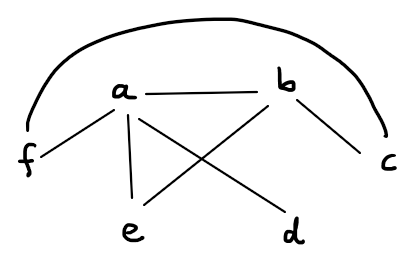
\includegraphics[height=5cm]{\pfad/Graphen/Aufgaben/visit_05/visit_05.png}

\ifprintanswers

\begin{lstlisting}
a  1 10
b  2  9
c  3  6
f  4  5
e  7  8
d  11 12
\end{lstlisting}

\fi
